\documentclass[a4paper, 11pt, oneside]{scrbook}

\usepackage[backend=biber]{biblatex}
\usepackage[ngerman]{babel}		
\usepackage[T1]{fontenc}	  	
\usepackage[utf8]{inputenc}
\usepackage[hidelinks]{hyperref}
\usepackage{graphicx}
\usepackage{epstopdf}
\usepackage{float}
\usepackage{acronym}
\usepackage{booktabs}
\usepackage{caption}
\usepackage{csquotes}
\usepackage{fancyhdr}
\usepackage{url}
\usepackage{hyperref}
\usepackage{blindtext}
\usepackage{wrapfig}
\usepackage{tcolorbox}
\usepackage{xcolor}

\renewcommand*{\headfont}{\normalfont}
\renewcommand*{\multicitedelim}{\addsemicolon\space}
\renewcommand*{\headrulewidth}{0pt}
\renewcommand*{\arraystretch}{1.5}

\setlength{\parskip}{1.5ex}
\raggedright

\bibliography{data/bibliography.bib}

\addbibresource{bibliography.bib}

\begin{document}

\frontmatter

\def\doctype{T3\_3101 Studienarbeit}
\def\title{Realisierung einer Plattform für Maschinelles Sehen auf Basis Docker mit PyTorch und YOLO}
\def\author{Tilmann Alexander Lorenz}

\begin{titlepage}

    \vspace{10mm}

    \begin{center}
        \vspace{5mm}

        \huge \title

        \vspace{14.2pt}

         \large \doctype


        \vspace{42.6pt}

        \vspace{42.6pt}

        \small des Studienganges Angewandte Informatik an der \\
        \large Dualen Hochschule Baden-Württemberg Mosbach

        \vspace{14.2pt}

        \includegraphics[height=1.5cm]{data/img/logo-dhbw.eps}

        \vspace{42.6pt}

        \small von \\
        \large \author
    \end{center}

    \vspace{98.6pt}

    \begin{table}[h]
        \centering
        \begin{tabular}{ll}
            \small Bearbeitungszeitraum           & 01.09.2022 - 16.06.2023                         \\
            \small Matrikelnummer, Kurs           & 2447899, INF20B                  \\
            \small Ausbildungsfirma               & Robert Bosch GmbH - Werk Bamberg \\
            \small Betreuer der Dualen Hochschule & Prof. Dr. Carsten Müller         \\
        \end{tabular}
    \end{table}

    \vspace{49.7pt}

    \fancypagestyle{empty}{
        \fancyhf{}
        \fancyfoot[C]{\today}
    }

\end{titlepage}

\tableofcontents

\chapter{Abkürzungsverzeichnis} 
\begin{acronym}
    \acro{yolo}[YOLO]{You Only Look Once Algorithm}
    \acro{hpc}[HPC]{High Performance Computer}
\end{acronym}

\listoffigures

\listoftables

\mainmatter

\nocite{*}
\chapter{Voraussetzungen}

Für eine erfolgreiche Installation der Umgebung auf dem Testsystem (für Development oder Debugging) sind folgende Sprachen/ Frameworks/ Pakete notwendig:
\begin{itemize}
    \item Python >= 3.9
    \item PyTorch $\rightarrow$ latest stable Version
    \item NVIDIA CUDA Toolkit $\rightarrow$ entsprechende Version (\textbf{muss NICHT die neuste sein})
    \item (\ac{yolo}v5)
\end{itemize}

Zum Zeitpunkt des Schreibens ist die neuste PyTorch Version 1.13.1. Dazu muss der entsprechende CUDA Compiler ausgesucht werden. Das wäre in diesem Fall die Version 11.6 und nicht die aktuellste CUDA Version. Es wird empfohlen nicht CUDA selber zu installieren, sondern dies mit PyTorch zusammen installieren. Installiert wird PyTorch zusammen mit CUDA mit:
\begin{verbatim}
    pip3 install torch torchvision torchaudio 
    --extra-index-url https://download.pytorch.org/whl/cu117
\end{verbatim}
Der Link kann je nachdem geändert werden, was für eine CUDA Version benötigt wird. Dies kann sich von der Version des NVIDIA Treibers abhängig sein.
\section{Probleme + Lösungen der Installation}

Bei der Installation kann es zu verschiedenen Probleme kommen, die zumindest beim Bearbeiten der Arbeit entstanden sind.

\textbf{Problem 1:} Der Dockercontainer Startet nicht.
\label{text:docker}
\textbf{Lösung:} 
\begin{enumerate}
    \item Das GitHub Repository von ultralytics \cite{glennjocher.2023} neu clonen 
    \item Das Dockerfile von \textit{./utils/docker/Dockerfile} in \textit{./} rein kopieren
    \item Dockerfile ausführen  (das kann je nach Anwendung eine sehr lange Zeit in Anspruch nehmen aufgrund der Größe)
    \item Dockercontainer starten
\end{enumerate}


\chapter{YOLO}
\label{sec:yolo}
\ac{yolo} ist ein populäres Objekt Erkennungsmodell, dass dafür bekannt ist besonders schnell und akkurat Objekte in Bildern zu erkennen. Dies liegt an der kleinen Modellgröße und den hohen Berechnungsgeschwindigkeiten. Des Weiteren nutzt \ac{yolo} das gesamte Bild als Trainingsgrundlage, was es sowohl ermöglicht Videos zu klassifizieren als auch die Fehlerrate reduziert, dass der Hintergrund als Teil des Objektes klassifiziert wird. In diesem Kapitel geht es darum wie die Schnittstelle bzw. der Algorithmus gefüttert werden muss und was der Algorithmus für Datenformate erwartet \cite{Jiang.2022}.

\begin{wrapfigure}{r}{5cm}
    \includegraphics[width=4cm]{data/img/ordnerstruktur_yolo.png}
    \caption{Ordnerstruktur für einen Datensatz}
    \label{fig:folderYolo}
\end{wrapfigure}

Für die Studienarbeit wird der YOLOv5 von ultralytics \cite{glennjocher.2023} genommenm, da diese folgende Vorteile bietet:
\begin{itemize}
    \item aktive Developer am Projekt
    \item große Community 
    \item Docker deployable
    \item CUDA- und GPU-Unterstützung
    \item Pytorch Beschleungigung
    \item viele Tutorials und Ressourcen für das Erlernen des Algorithmus
\end{itemize}


\section{Generelle Ordnerstruktur}
\label{sec:yolo_folderstructure}
Der \ac{yolo}-Algorithmus erwartet eine gewisse Ordnerstruktur. Diese muss eingehalten werden, damit der Algorithmus funktioniert. Ein Diagramm der Ordnerstruktur ist zu sehen in \autoref{fig:folderYolo}. Der hierarchisch gesehen höchste Ordner ist der Projektordner. Darin sollten alle Daten für den YOLO-Algorithmus enthalten sein. Dieser Ordner enthält die Trainings- und Testdateien. Optional kann auch ein Validierungsdatensatz enthalten sein und die \textit{.yaml} Datei.

Es wird empfohlen die \textit{.yaml} Datei in den Projektordner zu inkludieren. Der Aufbau der Datei wird in \autoref{sec:yaml_class} genauer beschrieben. Alle Dateien sind innerhalb des Projektordners einzugliedern.

Der Test, Train und Validordner müssen alle jeweils 2 Ordner besitzen mit dem Namen \textit{images} und \textit{labels}. Diese müssen auch über die verschiedenen Ordner exakt gleich, inklusive der Groß- und Kleinschreibung benannt sein.

Der \textit{images} Ordner enthält die entsprechenden Bilder. Zum Trainieren akzeptiert der \ac{yolo}-Algorithmus unter anderem die Bildformate \textit{png},\textit{jpg} und \textit{tiff}. Innerhalb des Ordners müssen alle Bilder einen einzigartigen Namen besitzen (es wird an dieser Stelle empfohlen, alle Bilder durchzunummerieren)

Der \textit{labels}-Ordner enthält die Label zu den entsprechenden Bildern in \textit{images}. Dabei müssen alle Label für ein entsprechendes Bild in einer gleichnamigen Textdatei mit der Endung \textit{.txt} unter dem Ordner \textit{labels} abgespeichert werden. Ein Beispiel: In dem Trainingsordner im Unterordner \textit{images} gibt es ein Bild mit dem Namen \textit{test.jpg}. Die dazugehörige Labeldatei wird im Ordner \textit{labels} unter dem Namen \textit{test.txt} gespeichert.

Im folgenden Abschnitt sollen nun der Aufbau einer solchen Labeldatei erläutert werden.

\section{Aufbau der Labeldatei}
Eine Labeldatei ist wie in \autoref{sec:yolo_folderstructure} definiert eine Textdatei mit entsprechendem Dateiname. Es wird empfohlen die Datei UTF-8 zu enkodieren. 

Jede Datei besteht aus einer unterschiedlichen Anzahl an Zeilen. Jede Zeile der Datei beschreibt ein Objekt, das in der Abbildung zu sehen ist. Es ist möglich, dass diese Bildbereiche eiinander überlappen. Eine Zeile ist wie folgt aufgebaut:
\begin{tcolorbox}
    \begin{verbatim}
        <class> <x-center> <y-center> <width> <height>
    \end{verbatim}
\end{tcolorbox}
\begin{figure}
    \begin{center}
        \includegraphics[width=8cm]{data/img/yolo_picture_structure.png}    
        \caption{Struktur YOLO Format veranschaulicht}
        \label{fig:yoloFormat}
    \end{center}
\end{figure}
\begin{itemize}
    \item \textless class\textgreater gibt die Klasse an des markierten Objektes. Klassen werden durch die \textit{.yaml}-Datei definiert. Gekennzeichnet wird diese durch eine Zahl. Weiteres in \autoref{sec:yaml_class}
    \item \textless x-center\textgreater $\rightarrow$ Angabe des Zentrums des Rechteckes in x-Richtung 
    \item \textless y-center\textgreater $\rightarrow$ Angabe des Zentrums des Rechteckes in y-Richtung 
    \item \textless width\textgreater $\rightarrow$ die Breite des Rechteckes bzw. des markierten Bereiches
    \item \textless height\textgreater $\rightarrow$ die Höhe des Rechteckes bzw. des markierten Bereiches
\end{itemize}
Ein Beispiel ist zu sehen in \autoref{fig:yoloFormat}. \textit{x\_center, y\_center, width, height} werden dargestellt als Verhältnis zur Gesamtlänge/-breite. Die Zahlen sind definiert durch $n\in[0,1]$.

Die Klassen werden im \textit{.yaml} Dateiformat definiert. Diese wird im folgenden Abschnitt genauer beleuchtet.

\section{YAML Klassifizierungsfile}
\label{sec:yaml_class}

Für jedes Projekt gibt es im Projektordner eine \textit{.yaml} Datei mit einem beliebigen Namen. Die \textit{.yaml}-Datei muss allerdings einem gewissen Aufbau folgen der folgend gezeigt wird. Dabei muss die Ordnerstruktur eingehalten werden wie in \autoref{fig:folderYolo} gezeigt:
\begin{verbatim}
    path: <path-to-project>
    train: <rel-path-to-train-dir>
    val: <rel-path-to-val-dir>

    names:
        0: <name>
        ...
\end{verbatim}
\begin{itemize}
\item \textless path-to-project\textgreater  $\rightarrow$ Absoluter Pfad zum Projektordner (inklusive des Projektordners)
\item \textless rel-path-to-train-dir\textgreater  $\rightarrow$ relativer Pfad zu den Bildern des Trainingsdatensatz ausgehend vom \textless path-to-project\textgreater-Pfad
\item \textless rel-path-to-val-dir\textgreater  $\rightarrow$ relativer Pfad zu den Bildern des Validierungsdatensatz ausgehend vom \textless path-to-project\textgreater-Pfad
\item \textit{names} $\rightarrow$ Liste aller Klassen und der Verbindung zwischen Name der Klasse angegeben durch \textless name\textgreater  und der Nummer. Die Nummer, beginnend mit 0 muss auch äquivalent sein zu der Nummerierung in den Textdateien. Der \ac{yolo}-Algorithmus assoziiert die Namen mit den Nummern durch die \textit{.yaml}-Datei
\end{itemize}

\chapter{Ausführen des Modells}
\section{Docker Setup und Vorbereitungen}
Damit der Docker Container funktioniert muss vorher Docker auf der Maschine installiert sein. Für weitere Informationen bitte Die Docker Dokumentation aufrufen: \textit{\href{https://www.docker.com/get-started/}{Siehe hier}}.

Wenn der Dockercontainer installiert wurde, kann der Dockercontainer auf 2 Weisen installiert werden. Entweder das folgende Kommando:

\begin{verbatim}
    docker pull ultralytics/yolov5
\end{verbatim}

Damit wird vom Dockerhub der ultralytics/yolov5 container gezogen und auf dem eigenen System installiert. Dies ist vor allem ratsam, wenn das Modell nicht geändert wird und der Algorithmus nicht geändert wird. Dabei wird es empfohlen dem \textit{\href{https://github.com/ultralytics/yolov5/wiki/Docker-Quickstart}{Quickstart}} von ultralytics zu folgen.

Die zweite Möglichkeit ist den Dockercontainer selber aufzubauen. Dies wurde bereits in \autoref{text:docker} erklärt. Hierbei ist der Vorteil, dass man noch zusätzlich den Dockercontainer beeinflussen kann und andere Anwendungen installieren oder den Dockercontainer mit anderen Anwendungen verknüpfen kann.

Wenn der Dockercontainer auf dem Zielsystem läuft, können die Daten kopiert werden.

\section{Daten kopieren}

Die Daten müssen wie in \autoref{sec:yolo} vorliegen und auf demselben System liegen, wo auch der Docker Container läuft. Dann kann man anschließend die Daten mit dem folgenden Befehl kopieren:

\begin{verbatim}
    docker cp <local_path> <docker_container_id>:<path_in_container>
\end{verbatim}

Erklärung:
\begin{itemize}
    \item \textless local\_path\textgreater ist der Pfad in dem System zu dem Basisordner des Datenpakets. Das Datenpaket ist ein Projekt beschrieben wie in \autoref{sec:yolo}. Dieser Pfad sollte den Basisordner mit einfügen. Wenn der Pfad zum Basisordner \textit{/usr/src/test-application/data} ist und der Basisordner heißt \textit{traffic}, dann ist der local\_path \textit{/usr/src/test-application/data/traffic}
    \item \textless docker\_container\_id\textgreater ist die ID des Contaioners. Dies ist nicht der Name. Zu sehen ist die, wenn man auf den Container klickt und sich die Details des Containers anzuschauen siehe \autoref{fig:doc_cont_term}
    \item \textless path\_in\_icontainer\textgreater dies ist der Pfad innerhalb des Containers am besten ist dies der Pfad des Working directorys + \textit{data}
\end{itemize}

\begin{figure}
    \centering
    \includegraphics[width=10cm]{data/img/docker_container_terminal.png}
    \caption{Docker Container ausschnitt mit der ID markiert in einem Roten Rahmen}
    \label{fig:doc_cont_term}
\end{figure}

Nach dem Kopieren der Daten muss das \textit{.yaml}-file im Base Folder noch unbenannt werden. Da der YOLO Algorithmus annimmt, dass das Beschreibungsskript nicht immer im selben Ordener liegt wie die daten muss der Pfad zu den Daten in das \textit{.yaml}-file eingeschrieben werden und das momentane Directory anstelle des \textit{/} eingesetzt werden.
\section{YOLO Modell Trainieren}
\label{sec:yolo_train}
Um das Modell zu trainieren sollte in den Docker Container gewechselt werden und das Terminal geöffnet werden. Mit dem Komando \textit{bash} wird in Bash gewechselt und es kann gesehen werden in welchem Ordner man sich befindet. 
\subsection{Befehlserklärung für Training des Modells}
Für das Training des Modells mus in das  Base Directory von dem YOLOv5 Repository gewechselt werden. Darin befindet sich die \textit{train.py} datei. Hierbei kann man das Training mit dem folgenden Befehl starten:
\begin{verbatim}
    python train.py --img <size_of_img> --batch <size_of_batches> --epochs <epochs>
    
    --data <data_path_to_yaml> --weights <weights> [--device <device_numbers> ]
\end{verbatim}
Die in eckickegen Klammern stehende Begriffe sollen nun nochmal erklärt werden:
\begin{itemize}
    \item \textless size\_of\_img\textgreater definiert die Breite des Bildes in Pixel. \textbf{Achtung:} Je höher der Pixelcount, desto höher der RAM / VRAM Verbrauch aber der Anstieg ist nicht linear, sondern Exponentiell
    \item \textless size\_of\_batch\textgreater gibt an wie viele Bilder in einem Durchgang (Epoche) analysiert werden soll. Diese kann per Hand vorgegeben werden, allerdings passiert es dann, dass aufgrund unzureichenden Videospeichers das Training abbricht. Für eine dynamische Anpassung des Videospeichers -1 eingeben. Allerdings kann es sein, dass dann alle Ressourcen genutzt werden.
    \item \textless epochs\textgreater gibt an wie oft trainiert wird. Für jede neue epoche werden die nächsten Batch an Images analysiert bis alle Bilder analysiert sind und der Algorithmus beginnt wieder von vorne. Somit wird sichergestellt, dass bei einer hohen Anzahl an Bildern alle Bilder untersucht werden.
    \item \textless weights\textgreater Für das Training gibt es 5 verschiedene Gewichte: Nano, Small, Medium, Large und XLarge. Für die jeweiligen Gewichte muss folgendes eingegeben werden. Es sei zu beachten, dass mit zunehmender größe die Rechendauer und der Platz an benötigten Arbeitsspeicher massiv zunimmt.
    \begin{itemize}
        \item Nano $\rightarrow $ \textit{yolov5n.pt}
        \item Small $\rightarrow $ \textit{yolov5s.pt}
        \item Medium $\rightarrow $ \textit{yolov5m.pt}
        \item Large $\rightarrow $ \textit{yolov5l.pt}
        \item XLarge $\rightarrow $ \textit{yolov5x.pt}
    \end{itemize}
    \item \textless device\_numbers\textgreater dies ist auch für die Arbeit ein optionaler Parameter. Dieser gibt an welche GPUs genutzt werden sollen. Wird, das ausgelassen geht der Algorithmus von einer CPU Berechnung aus und nutzt den vorliegenden Arbeitsspeicher und die CPU. Damit GPU(s) genutzt werden können müssen die Nummern der GPUs angegeben werden. Diese wird durch das Betriebssystem bestimmt. Wenn nur eine GPU vorhanden ist, ist dies i.d.R. 0. Damit wird der komplette VRAM der GPU genutzt. Voraussetzung dafür ist es, dass das NVIDIA CUDA Toolkit installiert ist und der GPU für den Docker freigeschaltet ist, was jedoch der default ist. Für mehrere GPUs einfach mit Kommata die GPUs auflisten. Für mehr Informationen \textit{\href{https://github.com/ultralytics/yolov5/issues/475}{hier klicken}}.
\end{itemize}

Falls diese Arbeit älter ist ein Jahr oder die bisherigen Angaben funktionieren nicht sei an dieser Stelle auf das Repository von ultralytics verwiesen, die eine ausführliche Dokumentation des Codes haben und all den wichtigen Befehlen.

\subsection{Nach Ausführung}
\label{sec:after_exec}
Nach der Ausführung sollte das Programm im ersten Schritt alle Trainingsdaten einlesen und anschließend je Epoche das Netz trainieren. Egal ob es fertig trainiert hat oder nicht wird in aufsteigender Reihenfolge im Working Directory unter \textit{./data/} zu finden sind. 

Wenn das Trainieren fehlgeschlagen sein sollte enthält der Ordner keine Gewichte. Gewichtsdateien sind mit der Endung \textit{.pt} gekennzeichnet.

Bei erfolgreichem TRainieren werden zwei Dateien Abelegt. Einmal \textit{latest.pt} und \textit{best.pt} die auf den jeweils zuletzt ausgeführten run und den besten run hinweisen. Diese können dann für die spätere Objekterkennung bzw. Ampel und Traffic Signs Erkennung genutzt werden.


\input{chapter/obj_detect.tex}
\chapter{Aufsetzen der Dockerumgebung}
Für das Aufsetzen der Dockerumgebung wurde der Hochleistungsrechner der DHBW Bad Mergentheim von Professor Doktor Carsten Müller genutzt. Für das Aufsetzen wurde dazu mit den vorgegebenen Passwörtern eingeloggt. 
\section{Aufsetzen der Installationsumgebungen}
Wichtig ist es zu schauen, dabei ob der Rechner zur Kommunikation mit dem Internet ein Proxy benötigt. Wenn dies der Fall ist folgende Befehle eingeben:

\begin{verbatim}
    sudo nano /etc/apt/apt.conf
\end{verbatim}
Darin müssen dann folgende Zeilen hinzugefügt werden:
\begin{verbatim}
    Acquire::http::Proxy "http://<adress>:<port>";
    Acquire::https::Proxy "https://<adress>:<port>";
\end{verbatim}
Die zweite Zeile muss nur hinzugefügt werden, wenn die Verbindung über eine verschlüsselte Verbindung geschehen sollen. Für den Fall, dass kein Proxy genutzt werden sollte, allerdings einer genutzt wird, müssen statt der obigen Zeilen in \textit{/etc/apt/apt.conf} folgende Zeilen einsetzen:
\begin{verbatim}
    Acquire::http::Proxy "false";
    Acquire::https::Proxy "false";
\end{verbatim}

\section{Aufsetzen Docker}
Für den Docker Container aufsetzen kann im generellen der Generellen Dockerdokumentation gefolgt zu werden zu finden \textit{\href{https://docs.docker.com/desktop/install/ubuntu/}{hier}}. Es kann durchaus sein, dass nach dem Folgen der Schritte die Fehlermeldung kommt, dass das Repository nicht gefunden werden konnte. Wenn dies der Fall ist, die nötigen SChritte rückwerts gehen und die verschiedenen Dateien wieder löschen und dem \textit{\href{https://www.digitalocean.com/community/tutorials/how-to-install-and-use-docker-on-ubuntu-20-04}{zweiten Tutorial}} folgen. Dies hatte in dieser Instanz geholfen das Docker Repository hinzuzufügen.
\chapter{Anleitung für Docker starten}
\section{Docker starten}
\begin{enumerate}
    \item Verbinden mit HPC 
    \item Unter \textit{/mnt/data/outside-data/} Ordner mit Namen Projekt anlegen für Studierenden (\textit{mkdir \textless Projektname\textgreater}) 
    \item Studierenden privaten Key vom Nutzer \textit{docker\_user} geben
    \item Studierende kopiert Daten auf \textit{/mnt/data/outside-data/} $\rightarrow$ die folgenden Schritte beziehen sich auf ein Windows Betriebssystem, für Linuxsysteme sind die ähnlichen Schritte nur die Berechtigungsschritte werden per \textit{chown 700 \textless user\textgreater \textless key\textgreater}
    
    \begin{enumerate}
        \item Studierende speichert Private Key auf PC ab
        \item Verbindung des PCs mit Mosbach VPN (Lehre Netz)
        \item Rechtsklick auf private Key im File Explorer $\rightarrow$ Properties $\rightarrow$ Sicherheit $\rightarrow$ erweitert $\rightarrow$ sollte Berechtigung sehen wie in \autoref{fig:berecht_1}
        \item klicken auf Vererbung Deaktivieren
        \item Hinzufügen klicken $\rightarrow$ SYSTEM suchen $\rightarrow$ Lese- und Execute und Schreibrechte geben $\rightarrow$ Ok klicken
        \item Hinzufügen klicken $\rightarrow$ \textless eigenen Nutzer\textgreater  suchen $\rightarrow$ Lese- und Execute und Schreibrechte geben $\rightarrow$ Ok klicken
        \item Danach sollte Berechtigung aussehen wie in \autoref{fig:berecht_2}
        \item Kommandozeile öffnen $\rightarrow$ wechseln in Directory wo Key legt
        \item Folgendes Kommando eingeben (alles eine Zeile)
        \begin{verbatim}
            scp -i <keyfile Name> -P 2022 <Pfad zu Datenablage>
            docker_user@193.197.11.229:/mnt/data/outside-data/<Name des Projektes>/  
        \end{verbatim}
        \item Information: \textless Pfad zu Datenablage\textgreater ist der Pfad zur Base Directory $\rightarrow$ alles darin wird rüberkopiert / \textless Name des Projektes\textgreater ist ein vorher angelegter Ordner, der den Namen des Projektes trägt, Password eingeben $\rightarrow$ wird von Herrn Müller übergeben
    \end{enumerate}
    \item Dockercontainer installieren $\rightarrow$ wenn Yolov5 bitte unten den Anweisungen folgen
    \item Client schließen und laufen lassen
\end{enumerate}

\begin{figure}
    \centering
    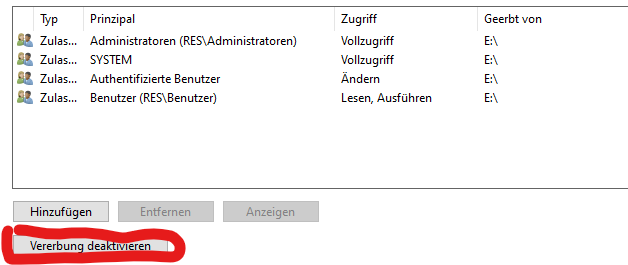
\includegraphics[width=8cm]{data/img/berechtigungen_1.png}
    \caption{Berechtigungen wie sie meistens voreingestellt sind durch Windows}
    \label{fig:berecht_1}
\end{figure}
\begin{figure}
    \centering
    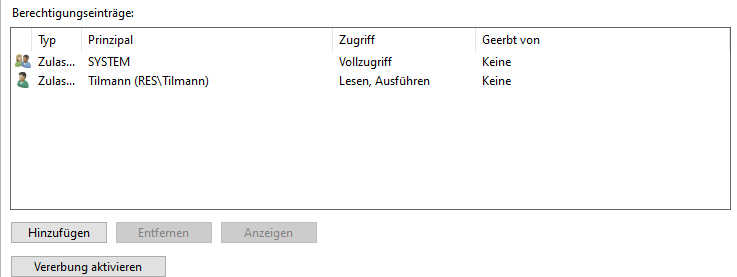
\includegraphics[width=8cm]{data/img/berechtigungen_2.png}
    \caption{Zielzustand Berechtigungen}
    \label{fig:berecht_2}
\end{figure}

\textbf{DIE FOLGENDEN SCHRITTE BEZIEHEN SICH AUSSCHLIEßLICH AUF YOLOv5}
\begin{enumerate}
    \item Entsprechenden Dockercontainer Pullen per Kommando: \textit{docker pull ultralytics/yolov5:latest} 
    \item eingeben Kommando unten (alles eine Zeile)
    \begin{verbatim}
        docker run --ipc=host -it --gpus all --memory="<memory limit>"
        --cpus="<cpu limit>" -v 
        /mnt/data/outside-data/<projektname>/:/usr/src/datasets
        ultralytics/yolov5:latest
    \end{verbatim}
    \begin{itemize}
        \item \textless memory limit\textgreater  wird eingegeben wie viel GB der Container nutzen darf, dabei immer nur das Vorzeichen Gigabyte  $\rightarrow$ g / Megabyte $\rightarrow$ m
        \item \textless cpu limit\textgreater gibt an wie viele CPUs maximal genutzt werden dürfen vom Container als Gleitkommazahl $\rightarrow$ 2 CPUs entspräche 2.0
        \item sowohl die gpus flag, memory flag als auch cpu flag dürfen weg gelassen werden, dann läuft der Container auf der gesamten Hardware    
    \end{itemize}
    \item wechseln in directory datasets und wechseln bis Base File des \textit{.yaml} gefunden wurde
    \item entsprechenden Base Path ändern um dem Pfad im Docker container zu repräsentieren
    \item wechseln in app directory
    \item eingeben Kommando: siehe \autoref{sec:yolo_train} und nach Angabe Studierenden
    \item client schließen

\end{enumerate}
Für weitere Information zu Yolov5 starten: \href{https://github.com/ultralytics/yolov5/wiki/Docker-Quickstart}{Link zu Yolov5 Starten} 

\section{Docker Container stoppen und löschen}
Zum Stoppen des Containers kann der folgende Befehl gesetzt werden:
\begin{verbatim}
    docker stop <container name>
\end{verbatim}
Der \textless Container name\textgreater kann durch den Befehl \textit{docker ps} angezeigt werden. Dabei wird in der letzten Spalte der Containername angezeigt und in der ersten Spalte die id. Stop funktioniert mit der Id.

Mit dem Befehl \textit{docker rm \textless Container id\textgreater} kann dann der Container gelöscht werden

\backmatter

\sloppy

\printbibliography

\end{document}